\documentclass{../../Latex_Template/Homework/homework}
\usepackage[utf8]{inputenc}
\usepackage{float}

% Graphics Path
\graphicspath{ {images/} }

\newcommand{\hwname}{Wu, Bo-Run}
\newcommand{\hwstudentid}{r08942073}
\newcommand{\hwnum}{3}
\newcommand{\hwtype}{Homework}
\newcommand{\hwsection}{}
\newcommand{\hwlecture}{}
\newcommand{\hwclass}{FinTech}
\newcommand{\hwdate}{2020-12-12}

\begin{document}

\maketitle

\question*{CNN}
  \begin{arabicparts}
    \questionpart
    I use two CNN layers and three DNN layers to construct the simple image
    classifier. I analyze the effect of both filter and stride size. The big
    filter size is used for large photos and capture more global features. For
    the stride size, small stride size is better at capturing more details of
    the photos.

    \questionpart 
    Figure \ref{fig:cnn_loss} is the loss of the CNN.
    \begin{figure}[H]
      \begin{center}
        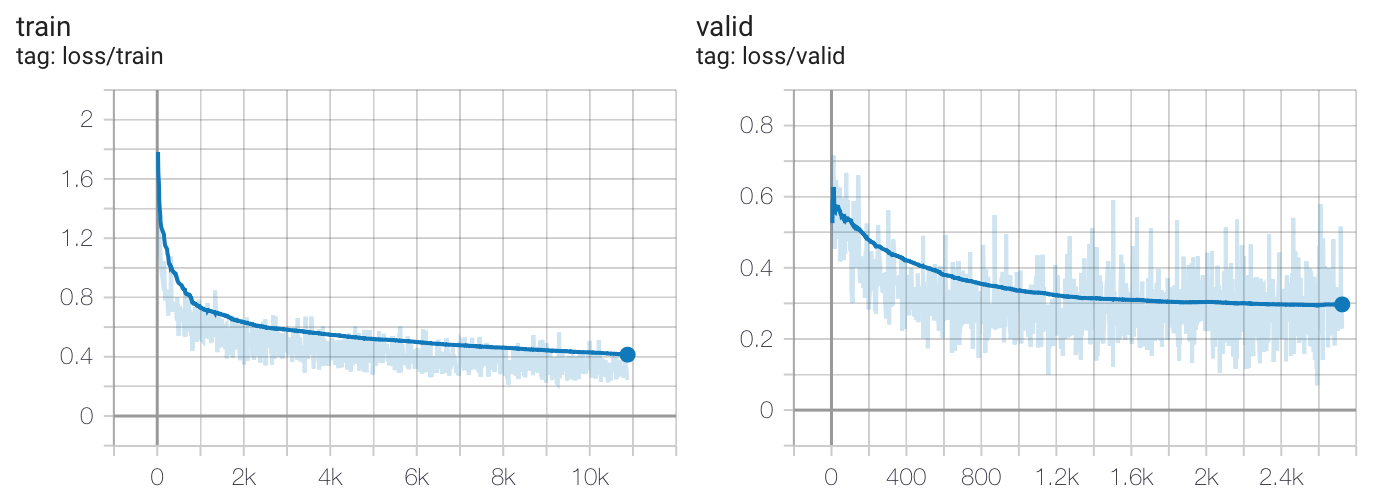
\includegraphics[width=0.5\linewidth]{CNN_loss.png}
        \caption{CNN Loss}
        \label{fig:cnn_loss}
      \end{center}
    \end{figure}

    Figure \ref{fig:cnn_accuracy} is the accuracy of the CNN.
    \begin{figure}[H]
      \begin{center}
        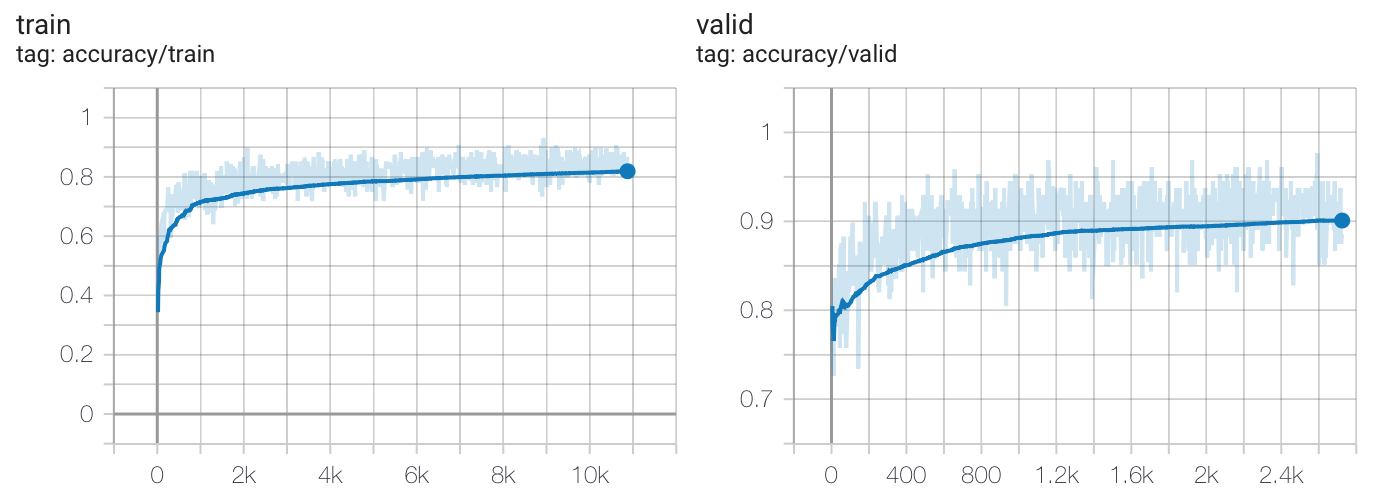
\includegraphics[width=0.5\linewidth]{CNN_accuracy.png}
        \caption{CNN Accuracy}
        \label{fig:cnn_accuracy}
      \end{center}
    \end{figure}

    \newpage

    \questionpart
    Figure \ref{fig:cnn_original} is the original photo and the label is Trouser.
    \begin{figure}[H]
      \begin{center}
        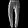
\includegraphics[width=0.5\linewidth]{CNN_original.png}
        \caption{CNN Original}
        \label{fig:cnn_original}
      \end{center}
    \end{figure}

    Figure \ref{fig:cnn_activation} is the output of the CNN first layer.
    \begin{figure}[H]
      \begin{center}
        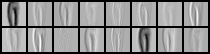
\includegraphics[width=0.5\linewidth]{CNN_activation.png}
        \caption{CNN Activation}
        \label{fig:cnn_activation}
      \end{center}
    \end{figure}

    \newpage

    \questionpart
    Figure \ref{fig:cnn_prediction} is the prediction of the CNN.
    \begin{figure}[H]
      \begin{center}
        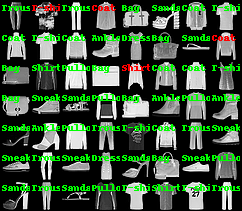
\includegraphics[width=0.5\linewidth]{CNN_predict.png}
        \caption{CNN Prediction}
        \label{fig:cnn_prediction}
      \end{center}
    \end{figure}

  \end{arabicparts}

\question*{AlexNet}
  \begin{arabicparts}
    \setcounter{partCounter}{1}
    \questionpart 
    Figure \ref{fig:alexnet_loss} is the loss of the AlexNet.
    \begin{figure}[H]
      \begin{center}
        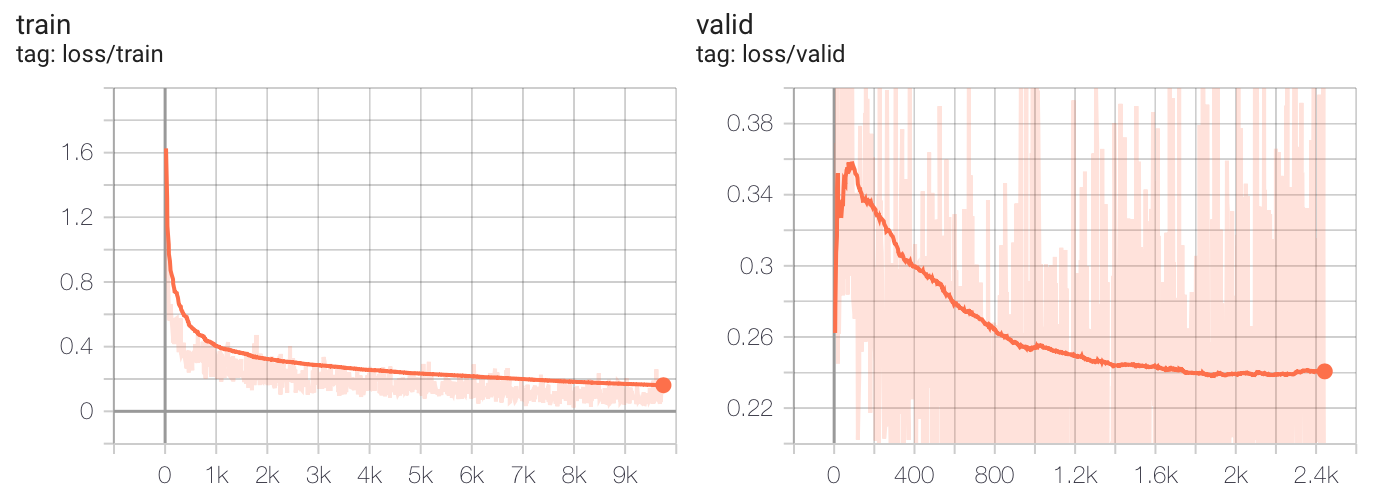
\includegraphics[width=0.5\linewidth]{Alexnet_loss.png}
        \caption{AlexNet Loss}
        \label{fig:alexnet_loss}
      \end{center}
    \end{figure}

    Figure \ref{fig:alexnet_accuracy} is the accuracy of the AlexNet.
    \begin{figure}[H]
      \begin{center}
        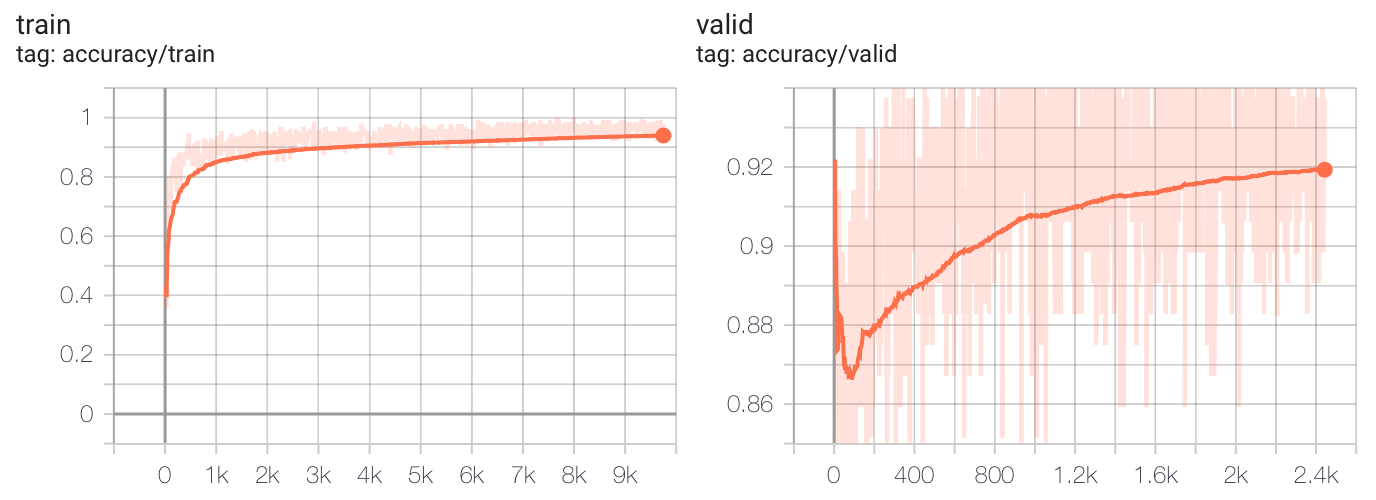
\includegraphics[width=0.5\linewidth]{Alexnet_accuracy.png}
        \caption{AlexNet Accuracy}
        \label{fig:alexnet_accuracy}
      \end{center}
    \end{figure}

    \questionpart
    Figure \ref{fig:alexnet_original} is the original photo and the label is
    Trouser.
    \begin{figure}[H]
      \begin{center}
        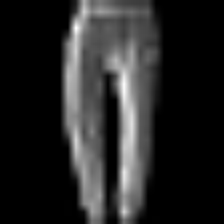
\includegraphics[width=0.5\linewidth]{Alexnet_original.png}
        \caption{AlexNet Original}
        \label{fig:alexnet_original}
      \end{center}
    \end{figure}

    Figure \ref{fig:alexnet_activation} is the output of the AlexNet first layer.
    \begin{figure}[H]
      \begin{center}
        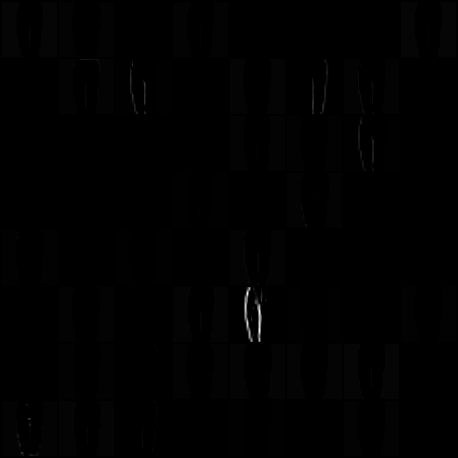
\includegraphics[width=0.5\linewidth]{Alexnet_activation.png}
        \caption{AlexNet Activation}
        \label{fig:alexnet_activation}
      \end{center}
    \end{figure}

    \questionpart
    Figure \ref{fig:alexnet_prediction} is the prediction of the AlexNet.
    \begin{figure}[H]
      \begin{center}
        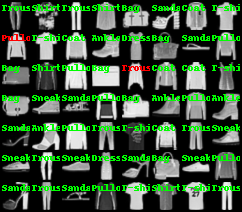
\includegraphics[width=0.5\linewidth]{Alexnet_predict.png}
        \caption{AlexNet Prediction}
        \label{fig:alexnet_prediction}
      \end{center}
    \end{figure}

  \end{arabicparts}

\end{document}
